\section{Evaluations} 
\begin{table*}[!t]
\footnotesize
\renewcommand{\arraystretch}{1.5}
\centering
\caption{\textbf{Performance of MiniMax-M1 on core benchmarks.}}
\setlength{\tabcolsep}{0.8mm}
\resizebox{\linewidth}{!}{
\begin{tabular}{c cccc | ccc | cc}
\toprule
\multirow{2}{*}{\textbf{Tasks}}
& \multicolumn{4}{c}{\textbf{Leading Close-Weights Models}}
& \multicolumn{3}{c}{\textbf{Open-Weights Models}}
& \multicolumn{2}{c}{\textbf{Our Models}} \\
\cmidrule(lr){2-5} \cmidrule(lr){6-8} \cmidrule(lr){9-10}
& \makecell{\textbf{OpenAI-o3}}
& \makecell{\textbf{Gemini 2.5} \\\textbf{Pro (06-05)}} 
& \makecell{\textbf{Claude} \\\textbf{4 Opus}}
& \makecell{\textbf{Seed-}\\\textbf{Thinking-}\\\textbf{v1.5}}
& \makecell{\textbf{DeepSeek-}\\\textbf{R1}}
& \makecell{\textbf{DeepSeek-}\\\textbf{R1-0528}}
& \makecell{\textbf{Qwen3-}\\\textbf{235B-A22B}}
& \makecell{\textbf{MiniMax-}\\\textbf{M1-40k}}
& \makecell{\textbf{MiniMax-}\\\textbf{M1-80k}} \\
\makecell{\scriptsize Extended\\\scriptsize Thinking}
& \makecell{\scriptsize \emph{100K}}
& \makecell{\scriptsize \emph{64K}}
& \makecell{\scriptsize \emph{64K}}
& \makecell{\scriptsize \emph{32K}}
& \makecell{\scriptsize \emph{32K}}
& \makecell{\scriptsize \emph{64K}}
& \makecell{\scriptsize \emph{32K}}
& \makecell{\scriptsize \emph{40K}}
& \makecell{\scriptsize \emph{80K}} \\
\midrule
\multicolumn{10}{c}{\emph{Mathematics}} \\
\hline
\makecell{AIME 2024}
& 91.6 & 92.0 & 76.0 & 86.7 & 79.8 & 91.4 & 85.7 & 83.3 & 86.0\\
\makecell{AIME 2025}
& 88.9 & 88.0 & 75.5 & 74.0 & 70.0 & 87.5 & 81.5 & 74.6 & 76.9\\
\makecell{MATH-500}
& 98.1 & 98.8 & 98.2 & 96.7 & 97.3 & 98.0 & 96.2 & 96.0 & 96.8 \\
\hline
\multicolumn{10}{c}{\emph{General Coding}} \\
\hline
\makecell{LiveCodeBench \\\emph{\tiny (24/8$\sim$25/5)}} & 75.8 & 77.1 & 56.6 & 67.5 & 55.9 & 73.1 & 65.9 & 62.3 & 65.0\\
\makecell{FullStackBench}
& 69.3 &   --   & 70.3 & 69.9 & 70.1 & 69.4 & 62.9 & 67.6 & 68.3\\
\hline
\multicolumn{10}{c}{\emph{Reasoning \& Knowledge}} \\
\hline
\makecell{GPQA Diamond}
& 83.3 & 86.4 & 79.6 & 77.3 & 71.5 & 81.0 & 71.1 & 69.2 & 70.0\\
\makecell{HLE \tiny\emph{ (no tools)}}
& 20.3 & 21.6 & 10.7 & 8.2  & 8.6$^*$  & 17.7$^*$ & 7.6$^*$ & 7.2$^*$ & 8.4$^*$\\
\makecell{ZebraLogic}
& 95.8 &  91.6  & 95.1 & 84.4 & 78.7 & 95.1 & 80.3 & 80.1 & 86.8\\
\makecell{MMLU-Pro}
& 85.0 & 86.0 & 85.0 & 87.0 & 84.0 & 85.0 & 83.0 & 80.6 & 81.1\\
\hline
\multicolumn{10}{c}{\emph{Software Engineering}} \\
\hline
\makecell{SWE-bench Verified} & 69.1 & 67.2 & 72.5 & 47.0 & 49.2 & 57.6 & 34.4 & 55.6 & 56.0\\
\hline
\multicolumn{10}{c}{\emph{Long Context}} \\
\hline
\makecell{OpenAI-MRCR} \emph{(128k)}
& 56.5 & 76.8 & 48.9 & 54.3 & 35.8 & 51.5 & 27.7 & 76.1 & 73.4 \\

\makecell{OpenAI-MRCR} \emph{(1M)} & -- & 58.8 & -- & -- & -- & -- & -- & 58.6 & 56.2 \\

\makecell{LongBench-v2} & 58.8 & 65.0 & 55.6 & 52.5 & 58.3 & 52.1 & 50.1 & 61.0 & 61.5 \\
\hline
\multicolumn{10}{c}{\emph{Agentic Tool Use}} \\
\hline
\makecell{TAU-bench \emph{(airline)}} & 52.0 & 50.0 & 59.6 & 44.0  & -- & 53.5 & 34.7 & 60.0 & 62.0\\
\makecell{TAU-bench \emph{(retail)}} & 73.9 & 67.0 & 81.4 & 55.7 & -- & 63.9 & 58.6 & 67.8 & 63.5\\
\hline
\multicolumn{10}{c}{\emph{Factuality}} \\
\hline
\makecell{SimpleQA} & 49.4 & 54.0 & -- & 12.9 & 30.1 & 27.8 & 11.0 & 17.9 & 18.5 \\
\hline
\multicolumn{10}{c}{\emph{General Assistant}} \\
\hline
\makecell{MultiChallenge} & 56.5 & 51.8 & 45.8 & 43.0 & 40.7 & 45.0 & 40.0 & 44.7 & 44.7 \\
\bottomrule
\multicolumn{10}{l}{\footnotesize * conducted on the text-only HLE subset.}
\end{tabular}
}
\label{tab:text-open-source-results-updated} % Changed label to avoid conflicts
\end{table*}
 

\subsection{Core Benchmarks} 


We conduct a comprehensive evaluation of MiniMax-M1 across several key domains: mathematics, general coding, software engineering, reasoning \& knowledge, long context, agentic tool use, factuality, and general assistant ability. We evaluate all tasks using temperature 1.0 and top-p 0.95 sampling.

\begin{itemize}
    \item \textbf{Mathematics:} To evaluate mathematical reasoning capabilities, we utilize several competition level math benchmarks, including MATH-500~\citep{hendrycks2021measuring},  AIME 2024, AIME 2025. For AIME evaluation, we sample 32 times and compute the average passrate as the final score.
    

     \item \textbf{General Coding:} We assess general programming proficiency using LiveCodeBench~\citep{jainlivecodebench} and FullStackBench~\citep{liu2024fullstackbenchevaluatingllms}, which evaluate code generation across diverse programming tasks. For both benchmarks, we report scores as the average passrate of 16 samples.
     
     \item \textbf{Reasoning \& Knowledge:} We assess domain knowledge and reasoning capabilities through GPQA-Diamond~\citep{rein2024gpqa}, MMLU-Pro~\citep{wang2024mmlu}, and the challenging HLE benchmark~\citep{phan2025humanity}. For GPQA-Diamond, we sample 32 times and report the average passrate.
     For HLE evaluation, we assess the model without external tools. Additionally, we measure logical reasoning ability using ZebraLogic~\citep{lin2025zebralogic}.

    \item \textbf{Software Engineering:} We evaluate software engineering capabilities using SWE-bench Verified~\citep{jimenez2024swebenchlanguagemodelsresolve}, which measures the ability to resolve real-world GitHub issues. We report results derived from the Agentless scaffold~\citep{xia2024agentless}. Departing from the original pipeline, our methodology employs a two-stage localization process (without any embedding-based retrieval mechanisms): initial coarse-grained file localization followed by fine-grained localization to specific files and code elements.
        
    % \item \textbf{Long Context:}
    \item \textbf{Long Context:} We evaluate long context understanding using OpenAI-MRCR~\citep{openai_mrcr}, which tests retrieval and disambiguation of multiple similar items within extended contexts, and LongBench-v2~\citep{bai2024longbench2}, a challenging benchmark with 503 multiple-choice questions across contexts ranging from 8k to 2M words.
    
    \item \textbf{Agentic Tool Use:} We assess tool use capabilities through TAU-bench~\citep{yaotau}, which emulates dynamic conversations where agents must utilize API tools while adhering to domain-specific policy guidelines. We evaluate TAU-bench with GPT-4.1 as user model, a general system prompt\footnote{"In each round, you need to carefully examine the tools provided to you to determine if any can be used. You must adhere to all of the policies. Pay attention to the details in the terms. Solutions for most situations can be found within these policies."} and without any custom tools. 
    The maximum number of interaction steps is 40. 
    % \emph{"In each round, you need to carefully examine the tools provided to you to determine if any can be used. You must adhere to all of the policies. Pay attention to the details in the terms. Solutions for most situations can be found within these policies."}

    \item \textbf{Factuality:} To measure factuality of LLMs, we utilize SimpleQA~\citep{wei2024measuring}, an adversarially-collected benchmark of fact-seeking questions with single, indisputable answers.

    \item \textbf{General Assistant:} We evaluate general assistant capabilities using MultiChallenge~\citep{sirdeshmukh2025multichallenge}, which assesses LLMs on conducting realistic multi-turn conversations with human users. We report our scores judged by GPT-4o. 
\end{itemize}


\noindent\textbf{Results on Math, Coding, and other General Tasks.}
 Table~\ref{tab:text-open-source-results-updated} presents our model's performance compared to state-of-the-art large reasoning models. In mathematical reasoning, the MiniMax-M1 models demonstrate strong performance across multiple benchmarks, achieving results comparable to the close-weight model Seed-Thinking-v1.5~\citep{seed2025seed1}. Notably, MiniMax-M1-80k achieves 86.0\% on AIME 2024, placing it second among open-weight models and trailing only the latest DeepSeek-R1-0528 model. For general coding, MiniMax-M1-80k matches Qwen3-235B on LiveCodeBench while outperforming it on FullStackBench, demonstrating robust capabilities among leading open-weight models.
On reasoning \& knowledge benchmarks, MiniMax-M1-80k similarly trails DeepSeek-R1-0528 but achieves competitive performance against other top open-weight models.
On the factuality benchmark SimpleQA, Minimax-M1 models underperform DeepSeek-R1 while outperforming all other open-weight models and Seed-Thinking-v1.5.
On MultiChallenge, both MiniMax models perform comparably to DeepSeek-R1-0528 and Claude 4 Optus, with inferior results only to o3 and Gemini-2.5-Pro.

\noindent\textbf{Highlights in Complex Scenarios: Software Engineering,  Long Context, and Tool use.}
Benefiting from our execution-based, software engineering environments during RL, MiniMax-M1-40k and MiniMax-M1-80k achieve strong scores of 55.6\% and 56.0\% on SWE-bench verified respectively. These results are slightly inferior to DeepSeek-R1-0528's 57.6\% and significantly surpass other open-weights models.
Leveraging its 1M context window, the M1 models significantly outperform all other open-weight models in long-context understanding. They even surpass OpenAI o3 and Claude 4 Opus, ranking second globally and trailing only Gemini 2.5 Pro by a small margin.
In agentic tool-use scenarios (TAU-bench), MiniMax-M1-40k surpasses all open-weight models and even Gemini-2.5 Pro. 
Moreover, MiniMax-M1-80k consistently outperforms MiniMax-M1-40k across most benchmarks, confirming the benefits of scaling test-time compute.



\begin{figure*}[t]
\begin{subfigure}[t]{0.32\textwidth}  % 注意这里用 [t]
    \centering
    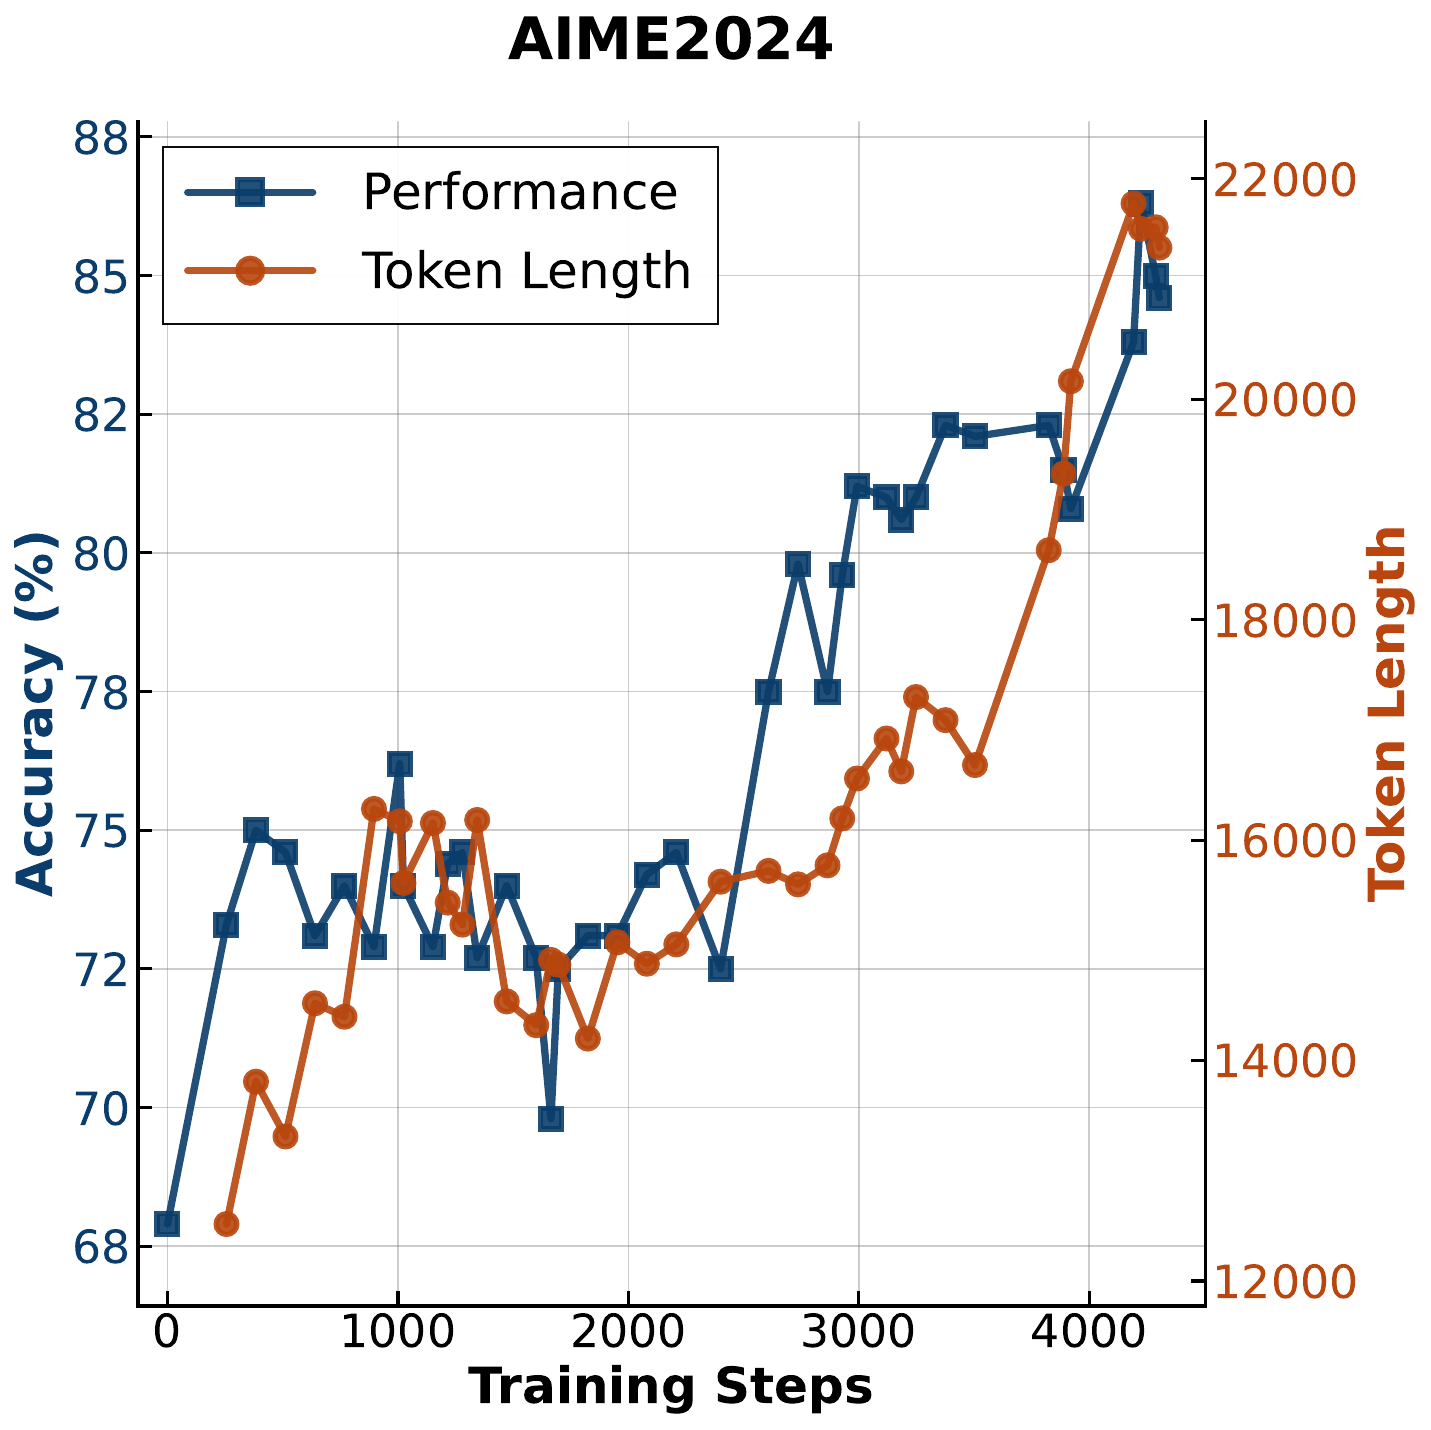
\includegraphics[width=\textwidth]{figures/figure5_scaling_dual_axis_aime24_test.pdf}
\end{subfigure}
\hfill
\begin{subfigure}[t]{0.32\textwidth}  % 这里也用 [t]
    \centering
    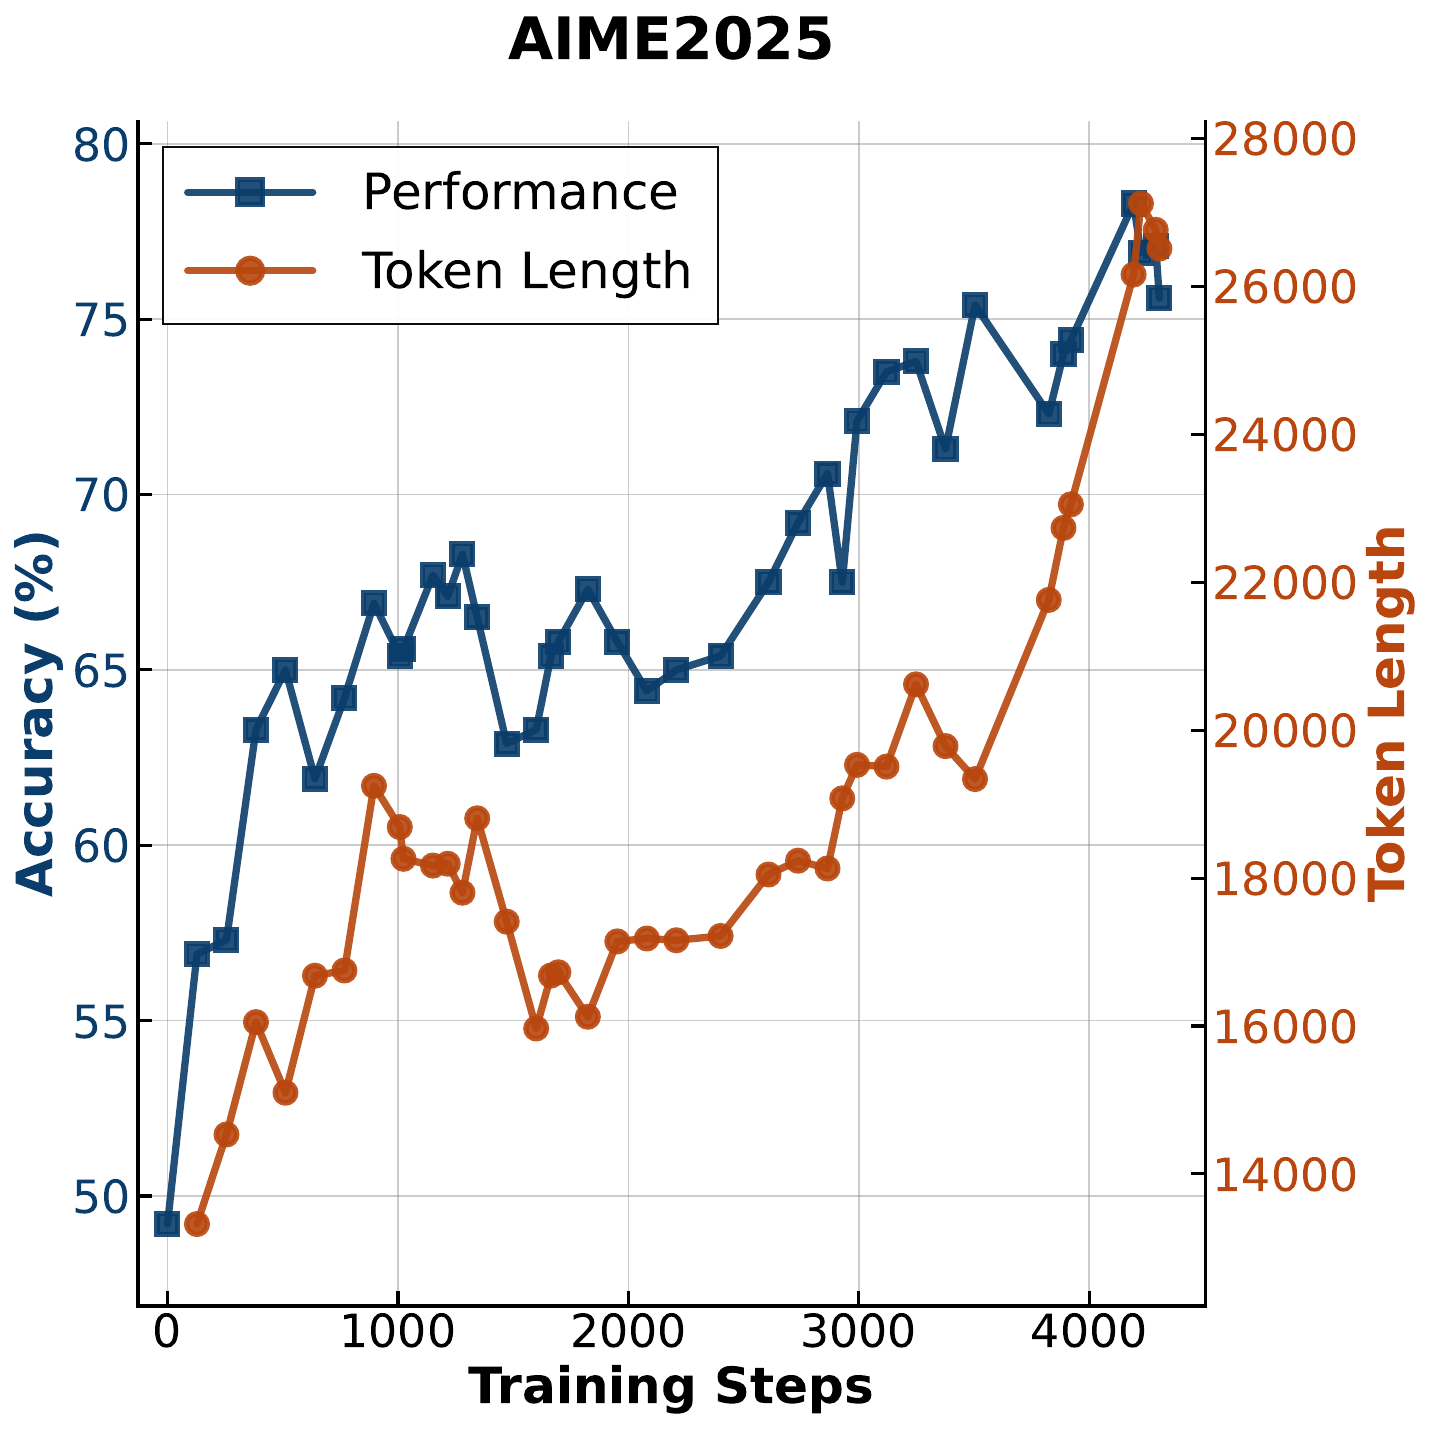
\includegraphics[width=\textwidth]{figures/figure5_scaling_dual_axis_aime25.pdf}
\end{subfigure}
\hfill
\begin{subfigure}[t]{0.32\textwidth}  % 这里也用 [t]
    \centering
    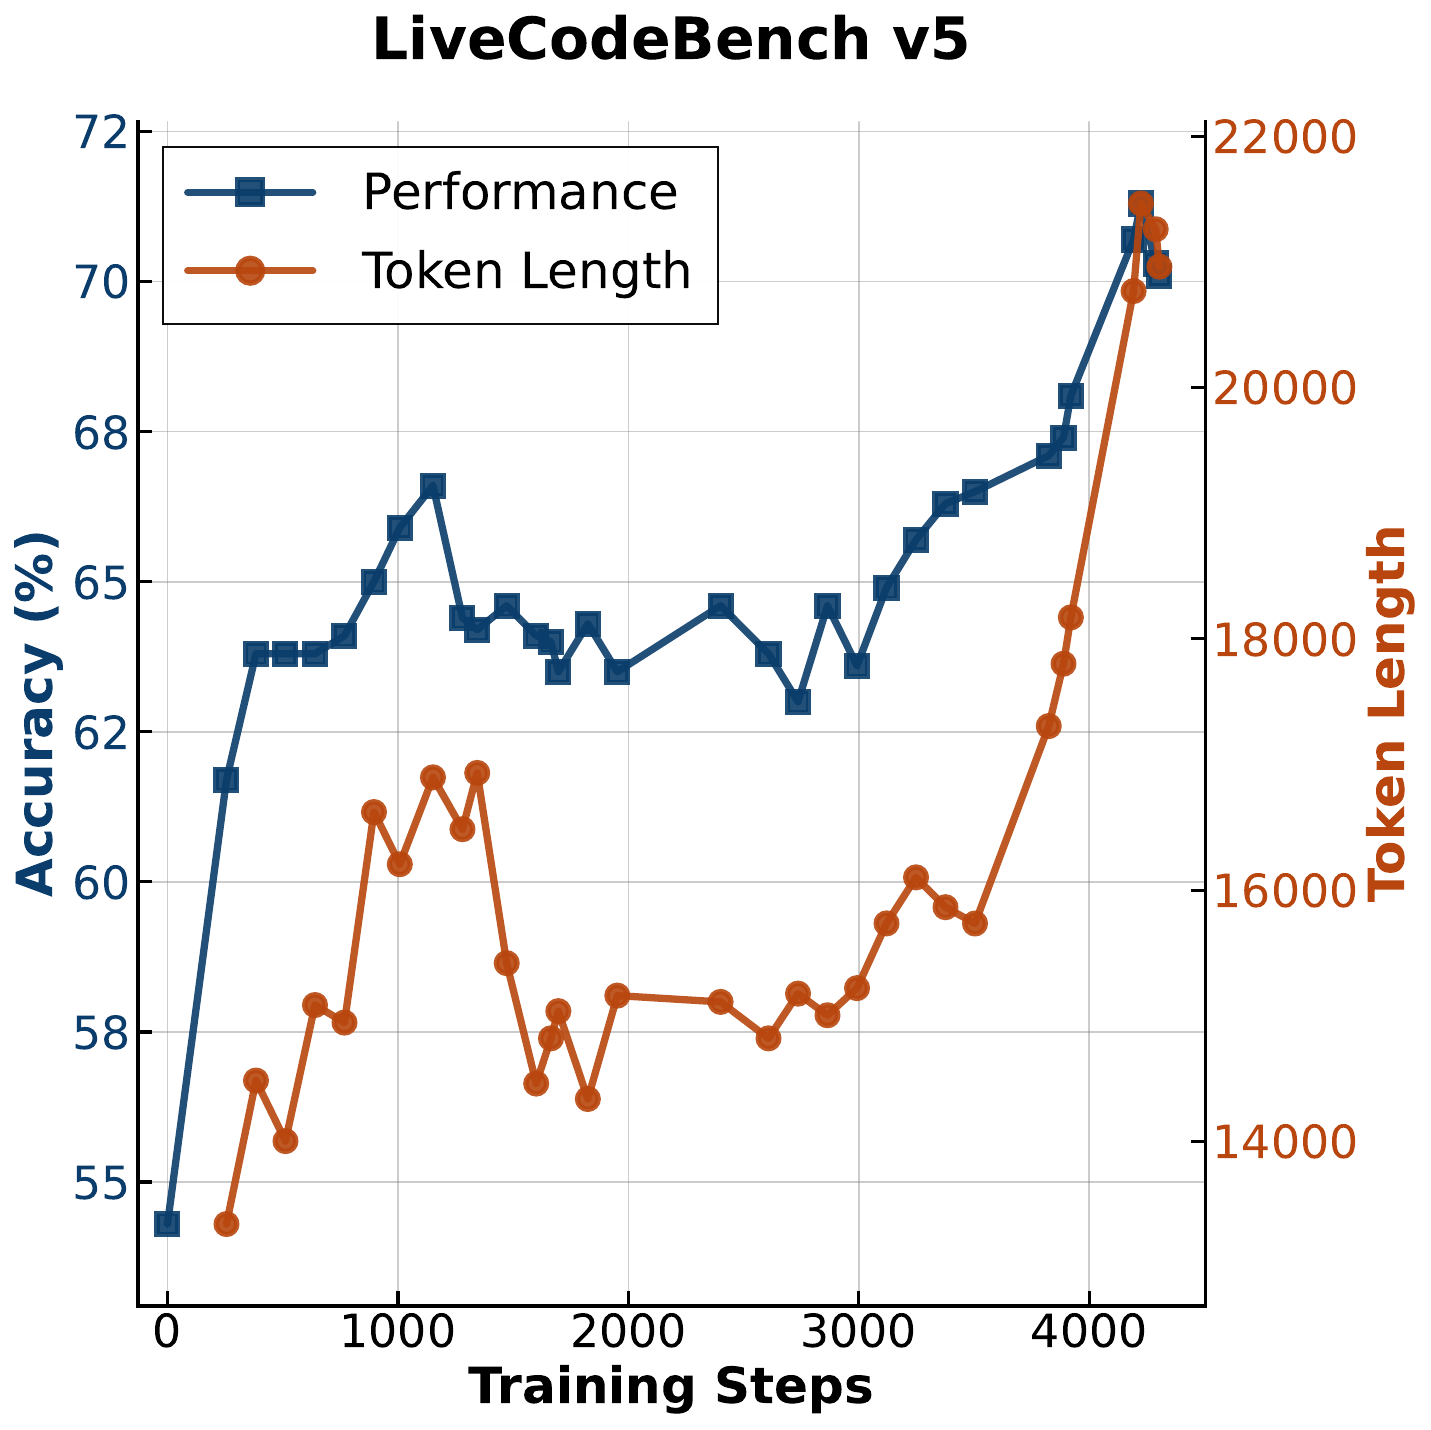
\includegraphics[width=\textwidth]{figures/figure5_lcb_scaling_dual_axis.pdf}
\end{subfigure}
\caption{Accuracy and generation length versus RL training steps for MiniMax-M1.}
\label{fig:scaling_results}
\end{figure*}

\subsection{Effect of RL Scaling}

To investigate the effect of RL scaling, we track performance and response length throughout training. Figure~\ref{fig:scaling_results} presents three representative examples from AIME 2024, AIME 2025, and LiveCodeBench v5, respectively. 
We observe consistent improvements in both model performance and response length during training. Notably, average response lengths on AIME and LiveCodeBench exceed 20,000 tokens, with AIME 2024 accuracy showing substantial gains from 68\% to 80\%. Crucially, the strong correlation between accuracy gains and increased response length in these visualizations underscores the importance of extending RL scaling to facilitate more extensive reasoning processes.
